\section*{Introduction}

PBImgAnalysis is a C library providing structures and functions to perform various data analysis on images.\\ 

It implements the following algorithms:
\begin{itemize}
\item K-means clustering on the RGBA space of pixels in a user defined radius
\end{itemize}

It uses the \begin{ttfamily}PBErr\end{ttfamily}, \begin{ttfamily}PBDataAnalaysis\end{ttfamily}, \begin{ttfamily}GenBrush\end{ttfamily} libraries.\\

\section{Interface}

\begin{scriptsize}
\begin{ttfamily}
\verbatiminput{/home/bayashi/GitHub/PBImgAnalysis/pbimganalysis.h}
\end{ttfamily}
\end{scriptsize}

\section{Code}

\subsection{pbimganalysis.c}

\begin{scriptsize}
\begin{ttfamily}
\verbatiminput{/home/bayashi/GitHub/PBImgAnalysis/pbimganalysis.c}
\end{ttfamily}
\end{scriptsize}

\section{Makefile}

\begin{scriptsize}
\begin{ttfamily}
\verbatiminput{/home/bayashi/GitHub/PBImgAnalysis/Makefile}
\end{ttfamily}
\end{scriptsize}

\section{Unit tests}

\begin{scriptsize}
\begin{ttfamily}
\verbatiminput{/home/bayashi/GitHub/PBImgAnalysis/main.c}
\end{ttfamily}
\end{scriptsize}

\section{Unit tests output}

\begin{scriptsize}
\begin{ttfamily}
\verbatiminput{/home/bayashi/GitHub/PBImgAnalysis/unitTestRef.txt}
\end{ttfamily}
\end{scriptsize}

\subsection{K-Means clustering on RGBA space}

imgkmeanscluster.tga:\\
\begin{center}
\begin{figure}[H]
\centering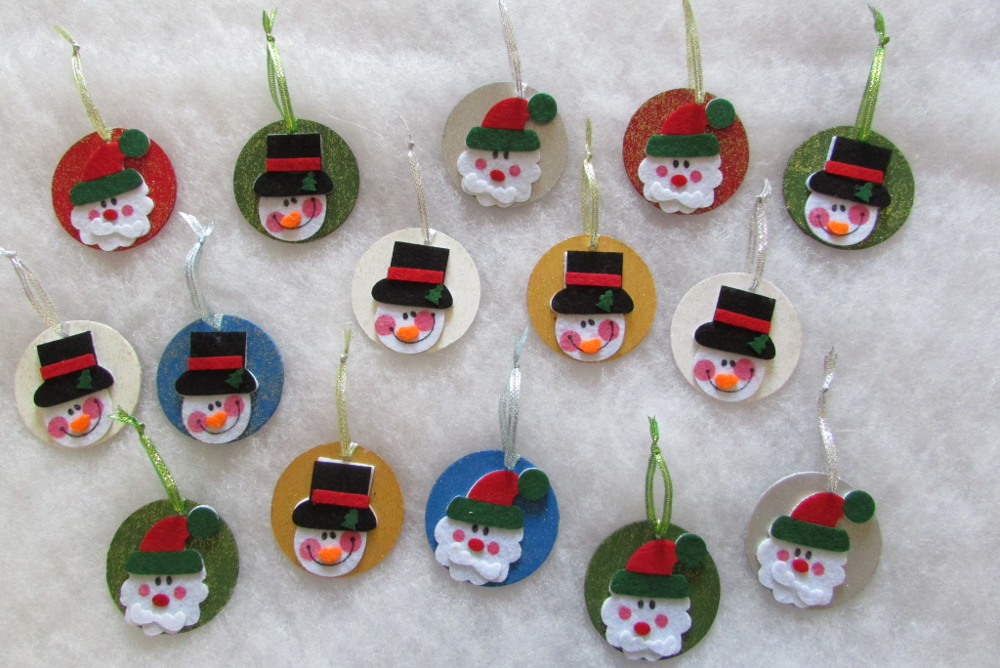
\includegraphics[width=6cm]{./imgkmeanscluster.png}\\
\end{figure}
\end{center}

clustering for K equals 2 to 6 and radius equals 0 to 5:\\
K=2:\\
\begin{center}
\begin{figure}[H]
\centering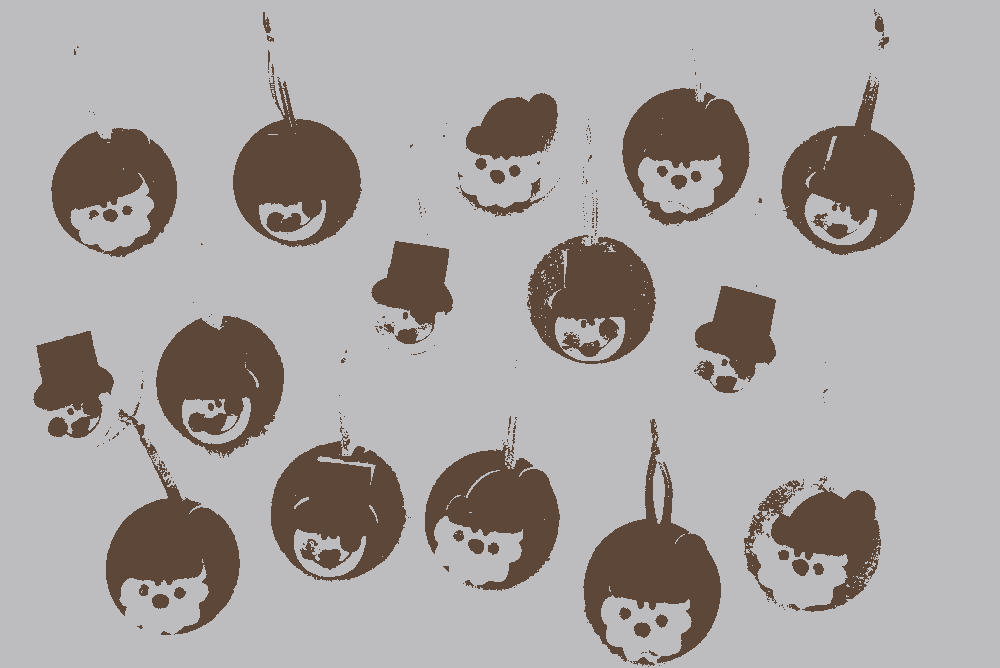
\includegraphics[width=6cm]{./imgkmeanscluster02-00.png}
\centering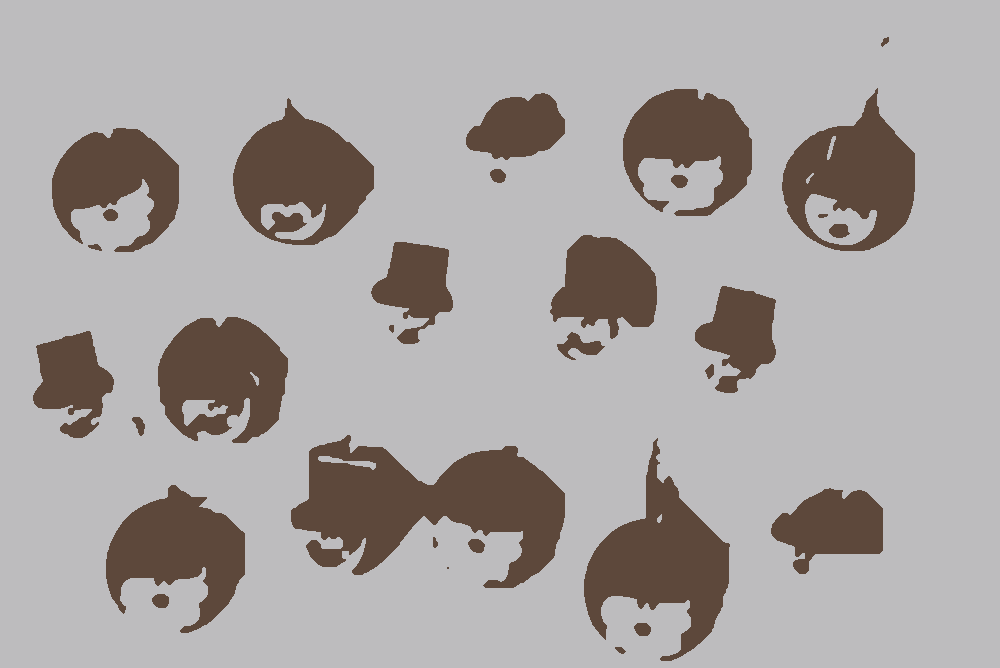
\includegraphics[width=6cm]{./imgkmeanscluster02-01.png}\\
\end{figure}
\end{center}
\begin{center}
\begin{figure}[H]
\centering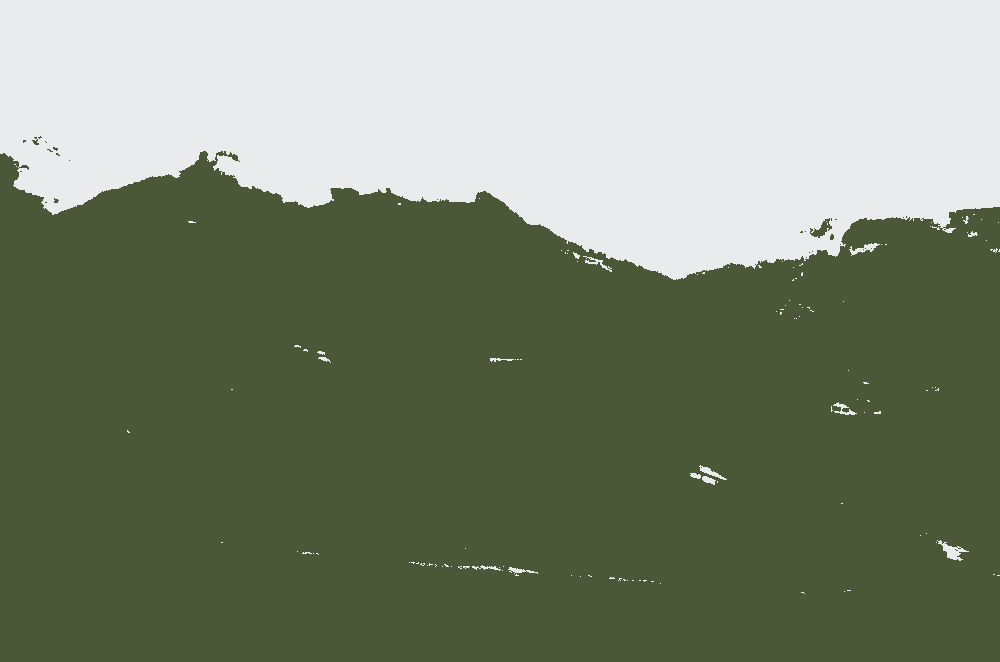
\includegraphics[width=6cm]{./imgkmeanscluster02-02.png}
\centering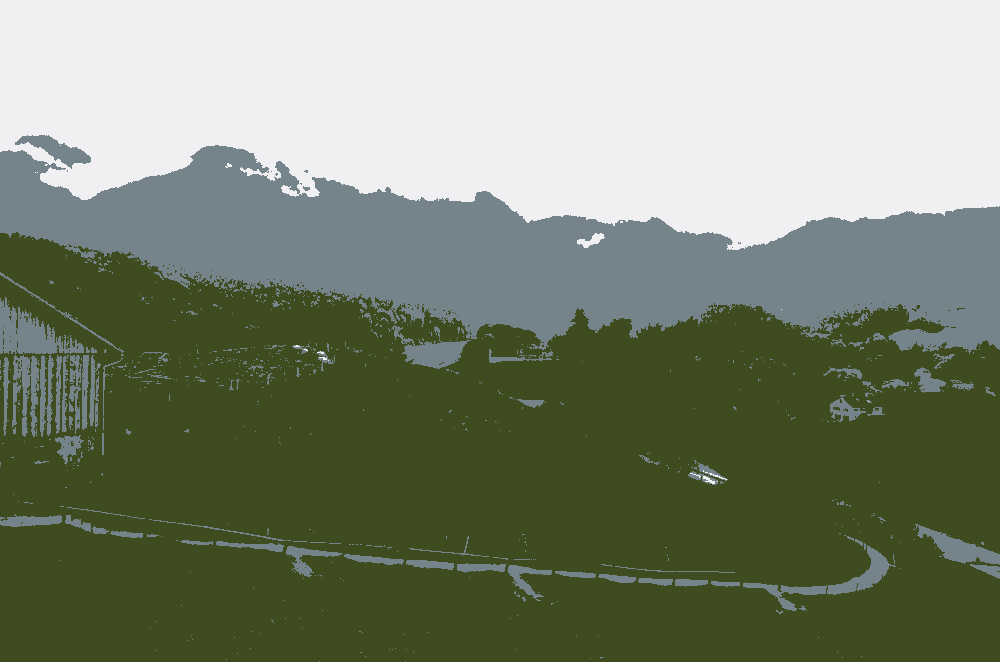
\includegraphics[width=6cm]{./imgkmeanscluster02-03.png}\\
\end{figure}
\end{center}
\begin{center}
\begin{figure}[H]
\centering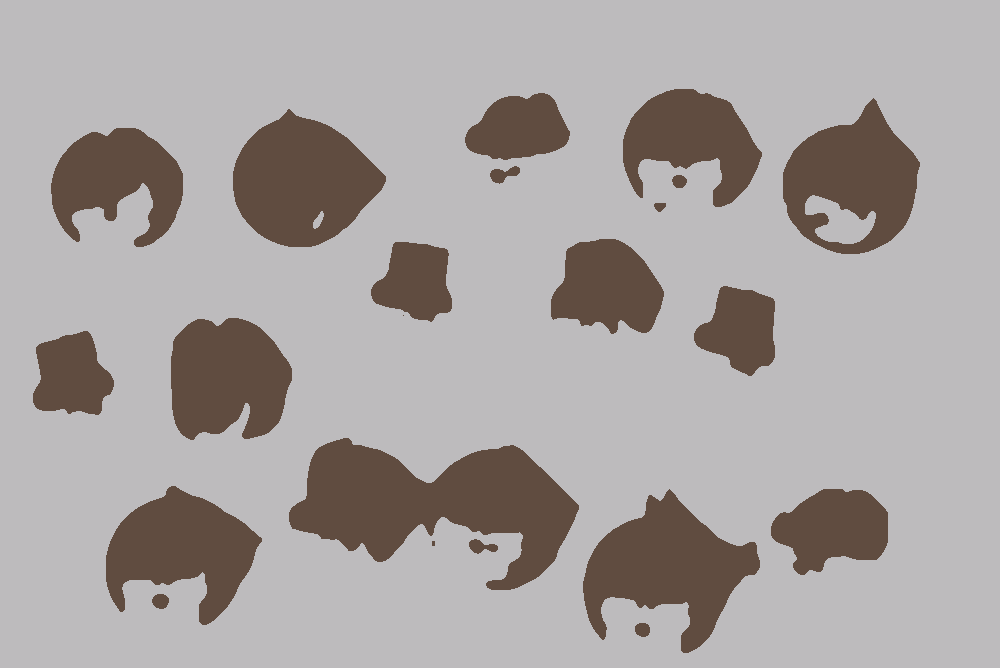
\includegraphics[width=6cm]{./imgkmeanscluster02-04.png}
\centering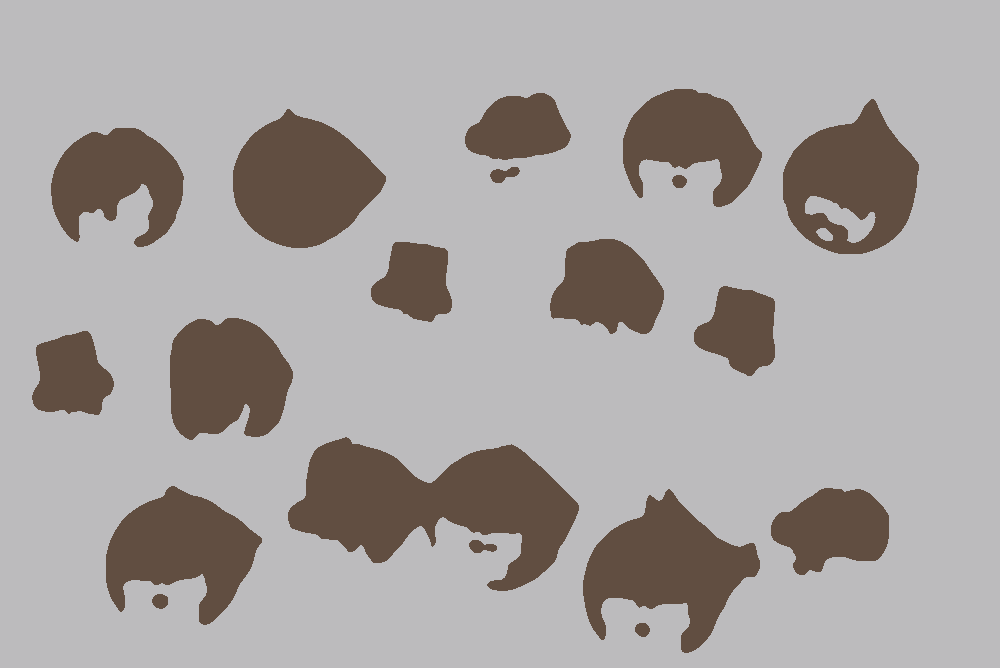
\includegraphics[width=6cm]{./imgkmeanscluster02-05.png}\\
\end{figure}
\end{center}
K=3:\\
\begin{center}
\begin{figure}[H]
\centering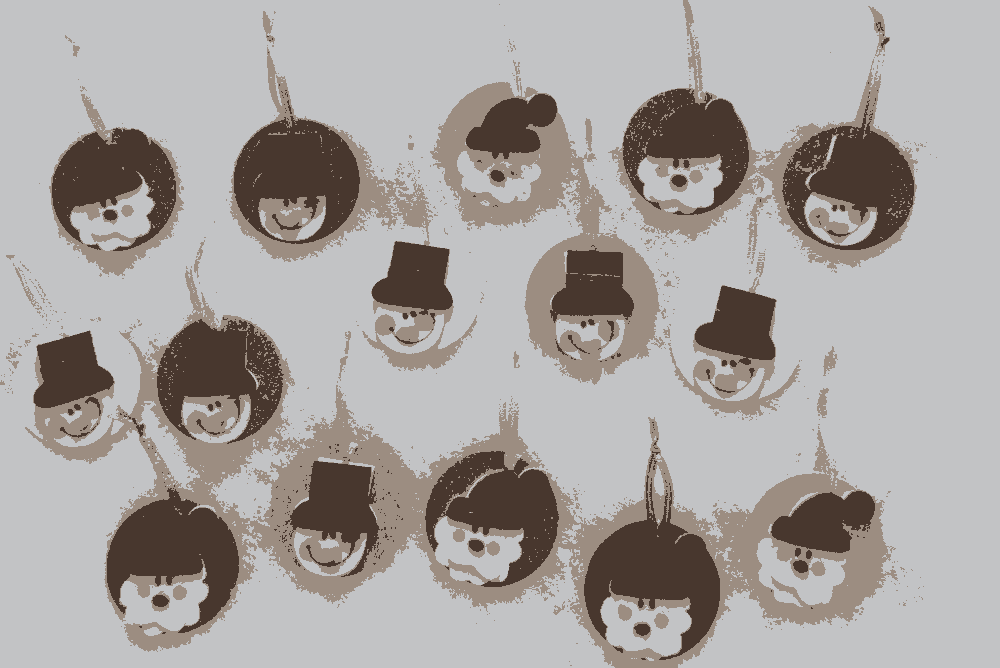
\includegraphics[width=6cm]{./imgkmeanscluster03-00.png}
\centering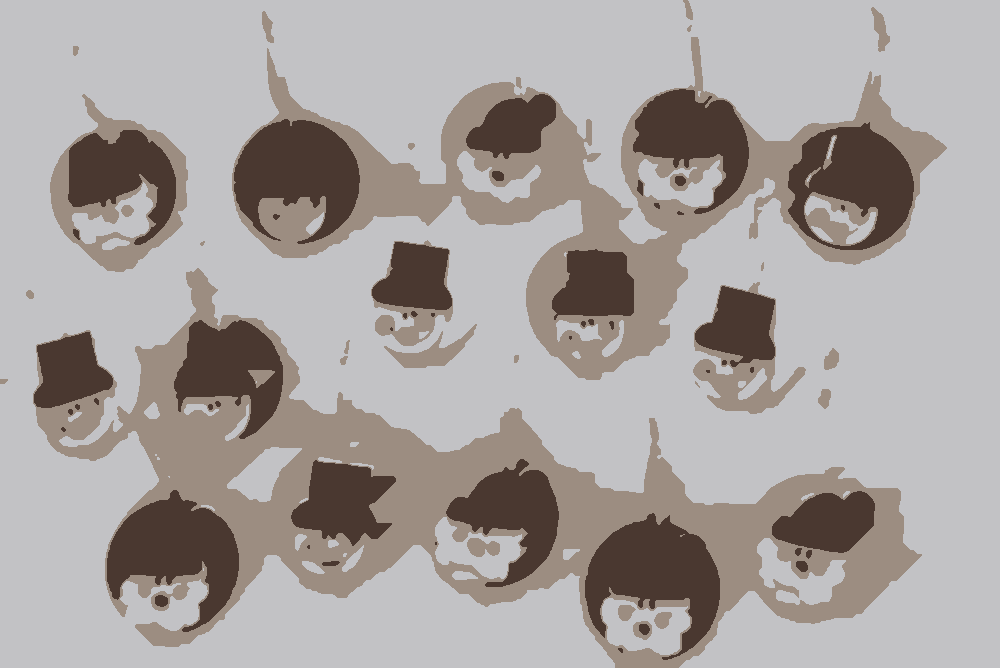
\includegraphics[width=6cm]{./imgkmeanscluster03-01.png}\\
\end{figure}
\end{center}
\begin{center}
\begin{figure}[H]
\centering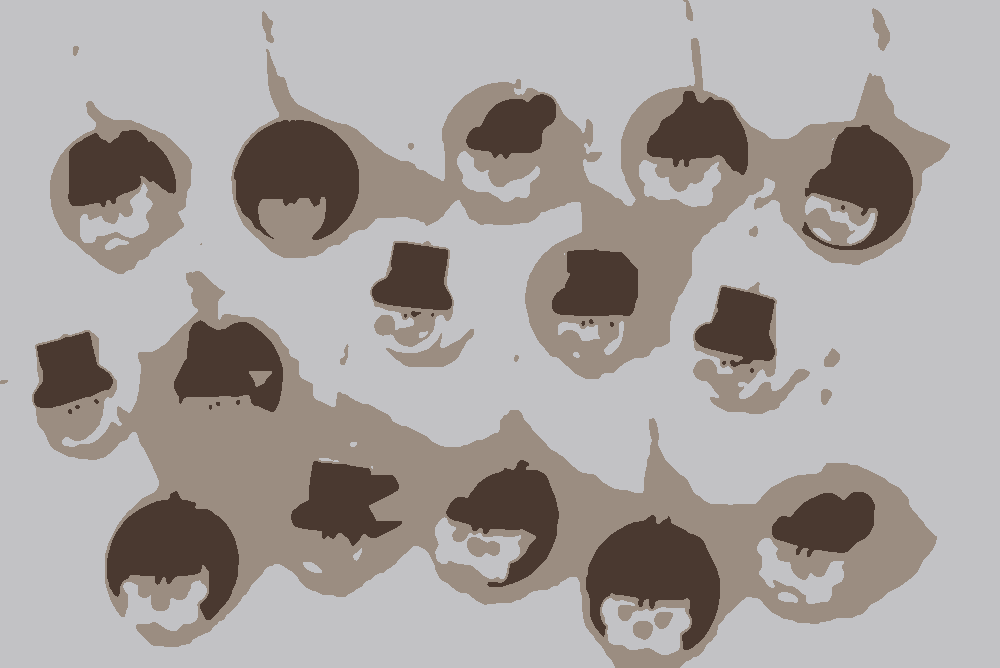
\includegraphics[width=6cm]{./imgkmeanscluster03-02.png}
\centering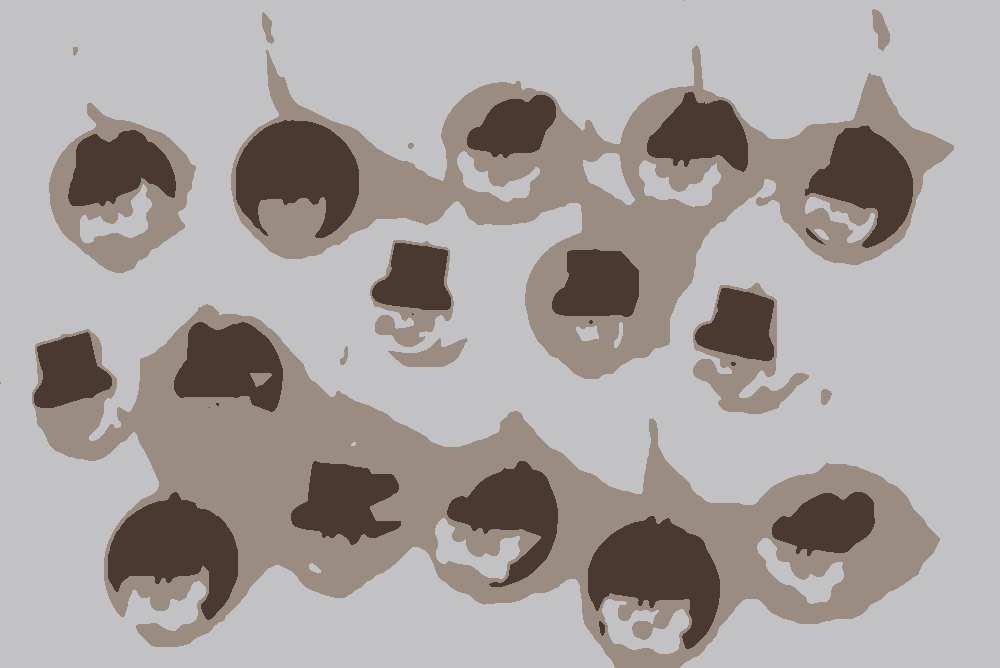
\includegraphics[width=6cm]{./imgkmeanscluster03-03.png}\\
\end{figure}
\end{center}
\begin{center}
\begin{figure}[H]
\centering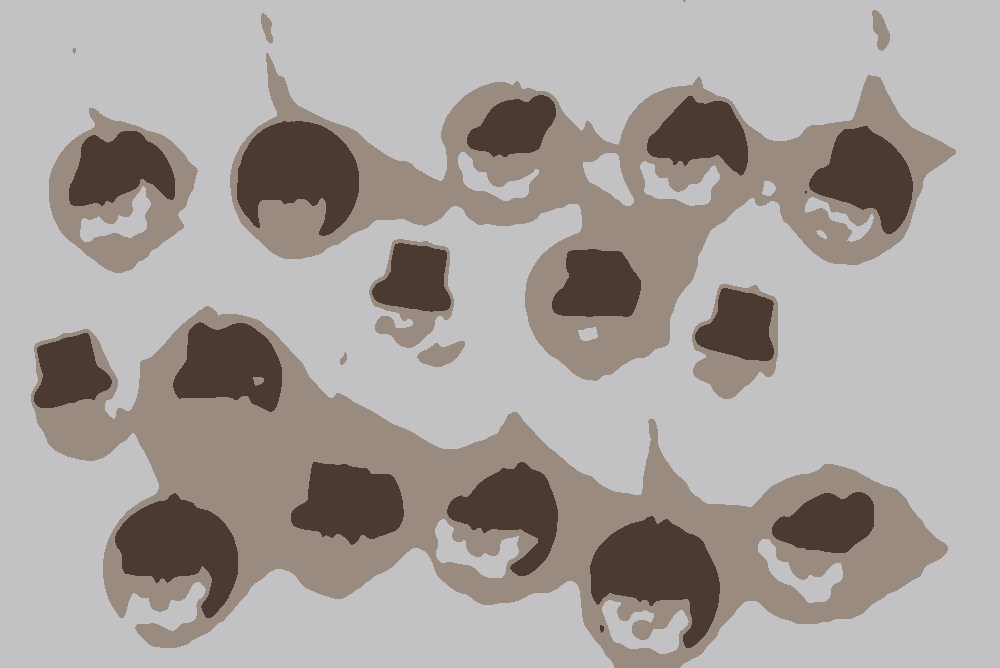
\includegraphics[width=6cm]{./imgkmeanscluster03-04.png}
\centering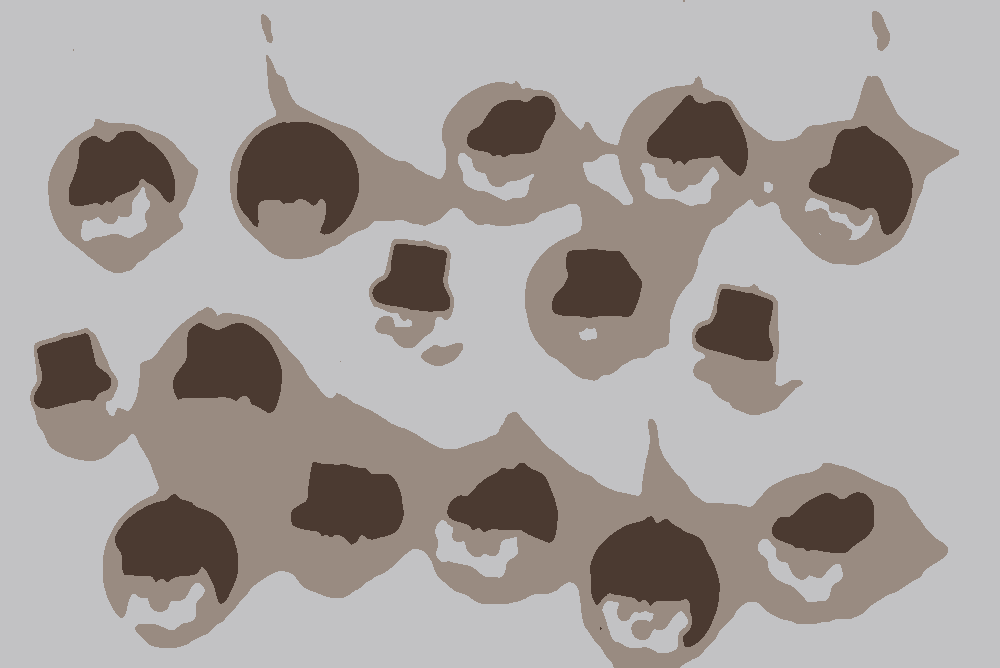
\includegraphics[width=6cm]{./imgkmeanscluster03-05.png}\\
\end{figure}
\end{center}
K=4:\\
\begin{center}
\begin{figure}[H]
\centering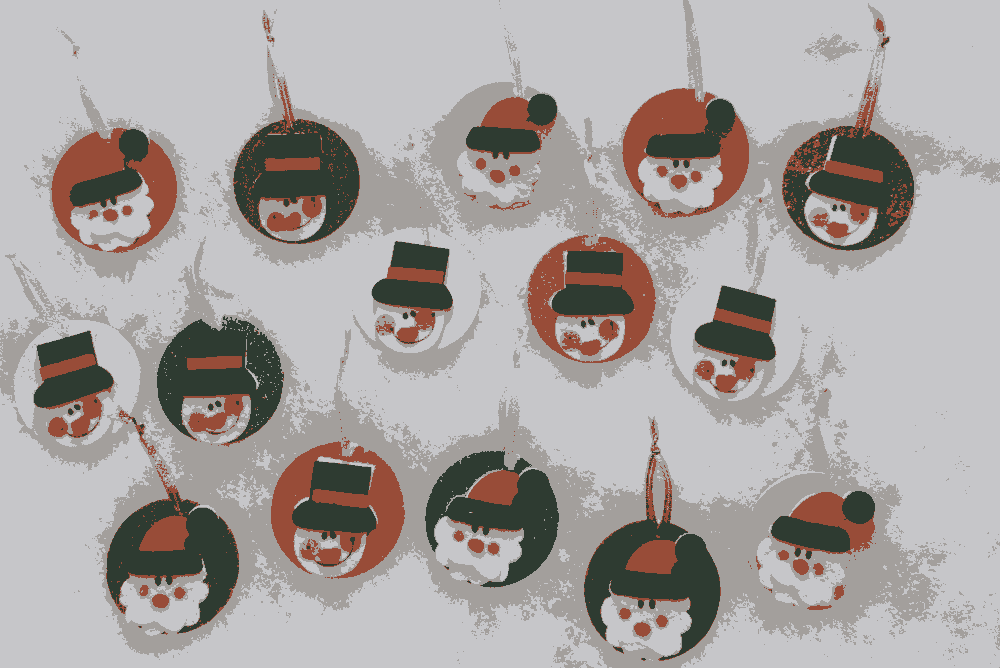
\includegraphics[width=6cm]{./imgkmeanscluster04-00.png}
\centering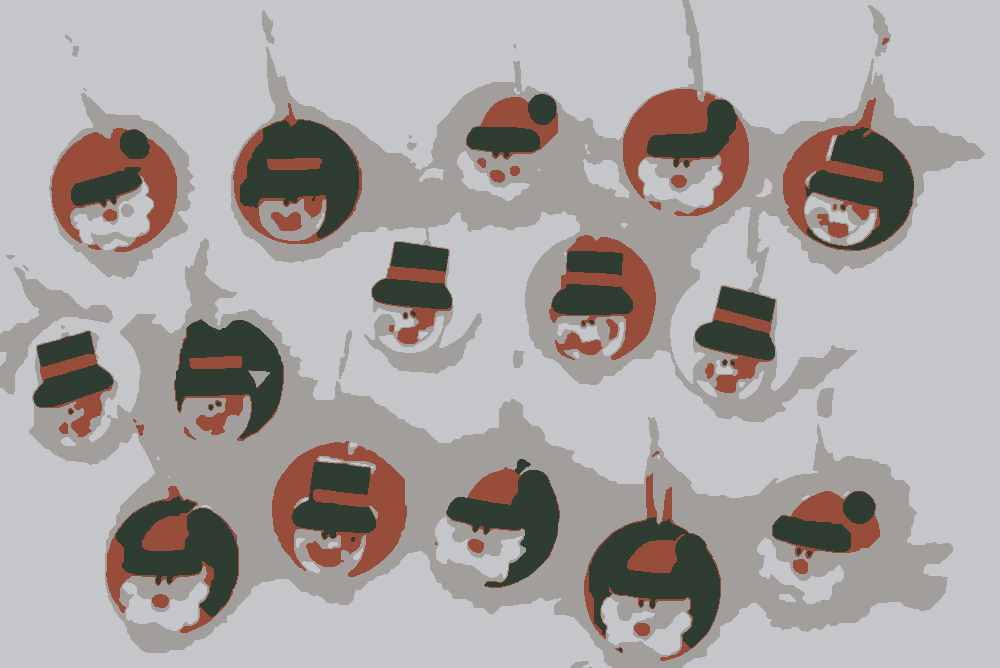
\includegraphics[width=6cm]{./imgkmeanscluster04-01.png}\\
\end{figure}
\end{center}
\begin{center}
\begin{figure}[H]
\centering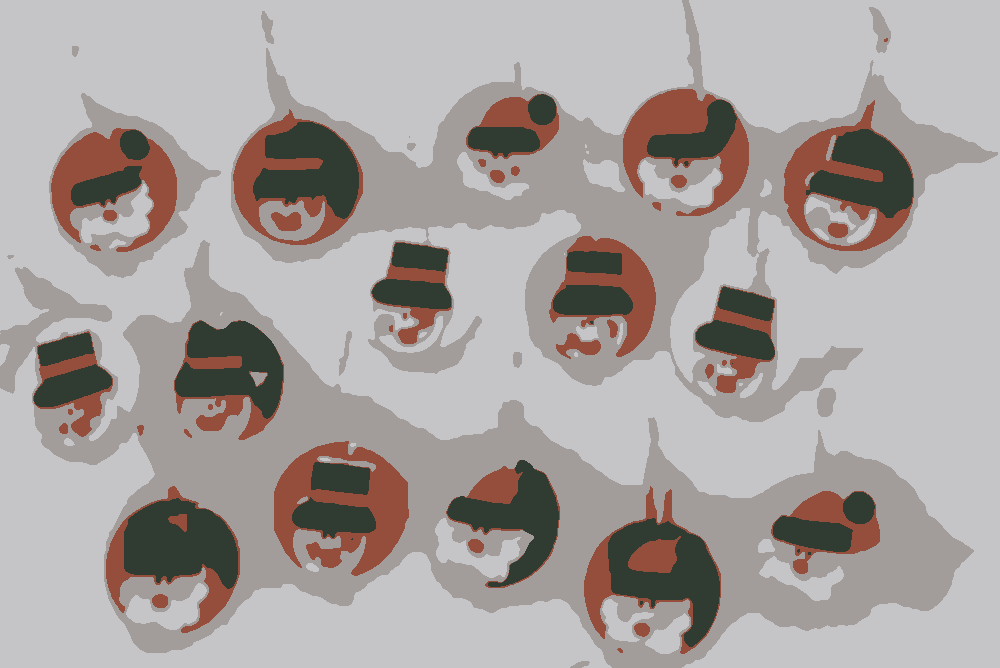
\includegraphics[width=6cm]{./imgkmeanscluster04-02.png}
\centering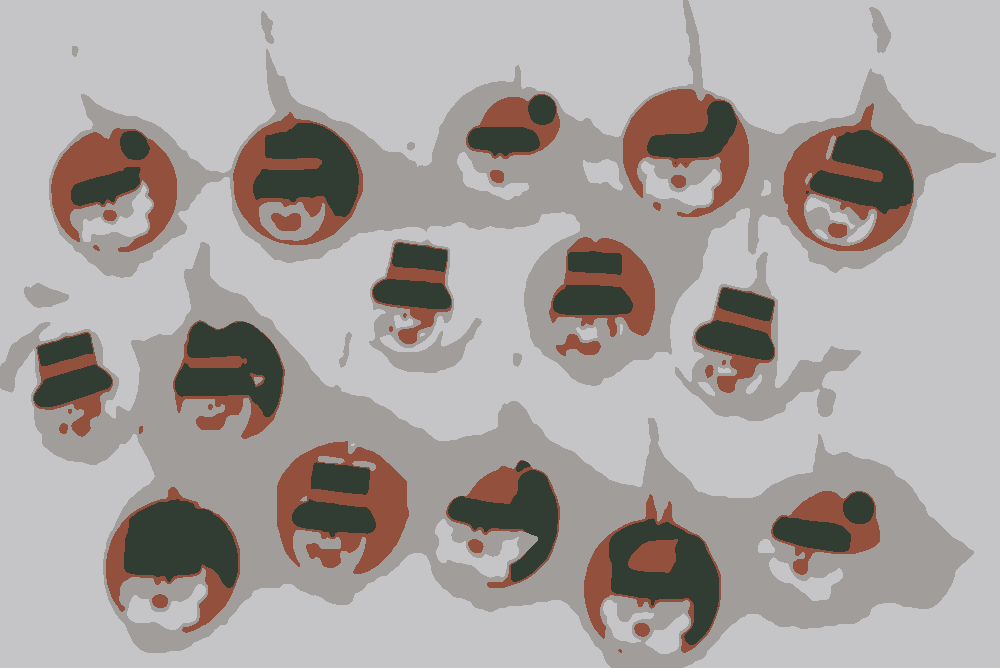
\includegraphics[width=6cm]{./imgkmeanscluster04-03.png}\\
\end{figure}
\end{center}
\begin{center}
\begin{figure}[H]
\centering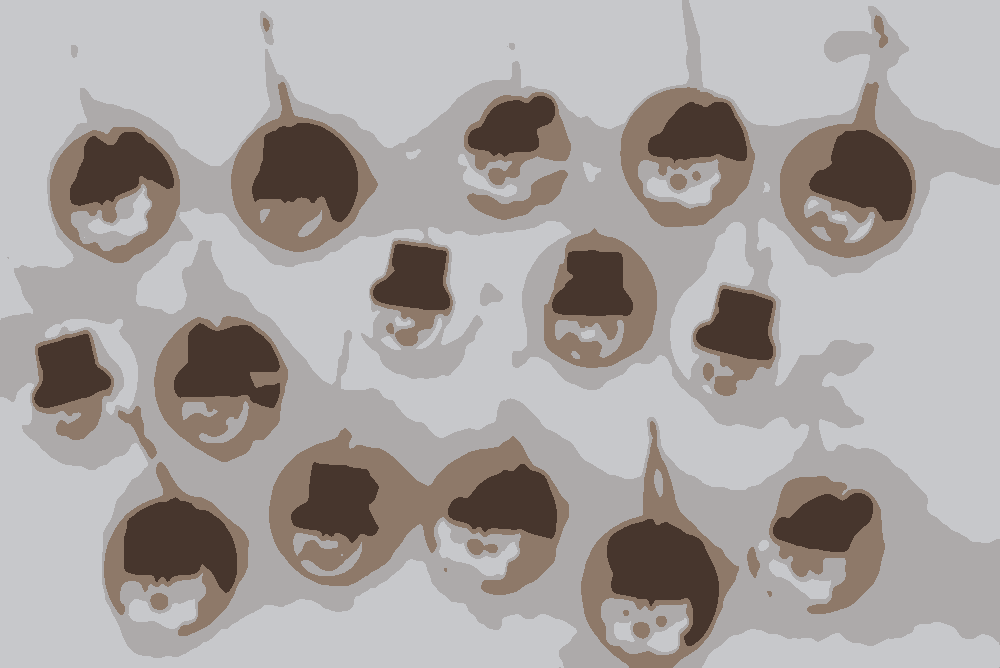
\includegraphics[width=6cm]{./imgkmeanscluster04-04.png}
\centering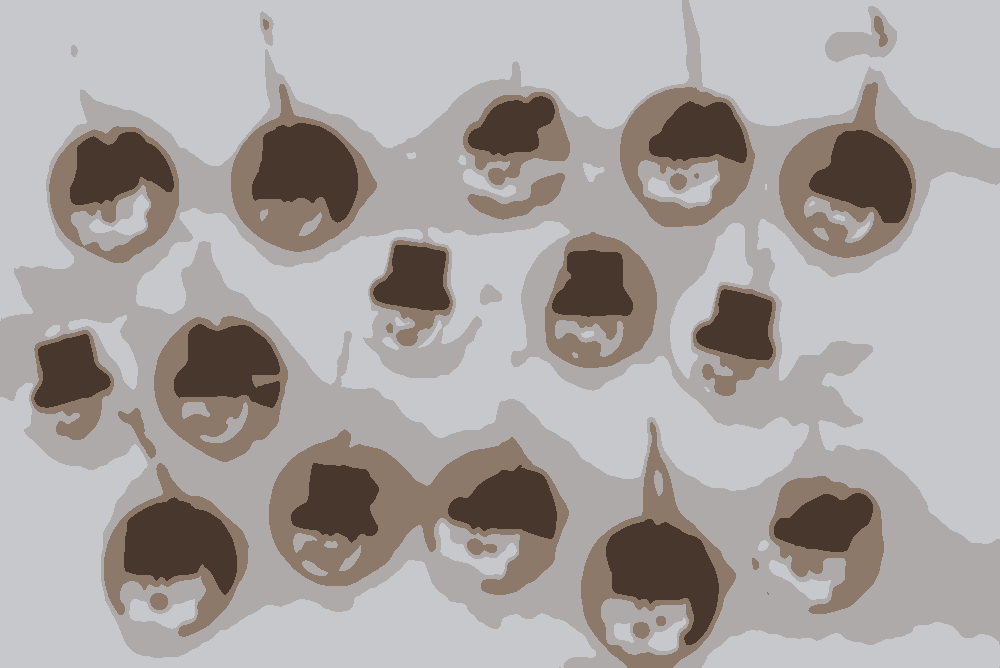
\includegraphics[width=6cm]{./imgkmeanscluster04-05.png}\\
\end{figure}
\end{center}
K=5:\\
\begin{center}
\begin{figure}[H]
\centering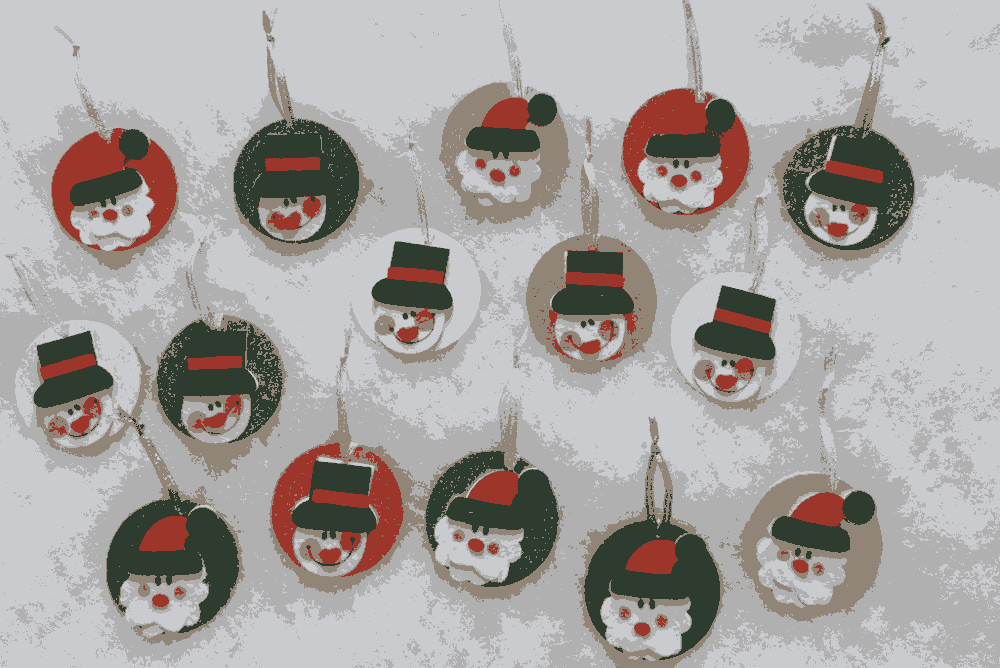
\includegraphics[width=6cm]{./imgkmeanscluster05-00.png}
\centering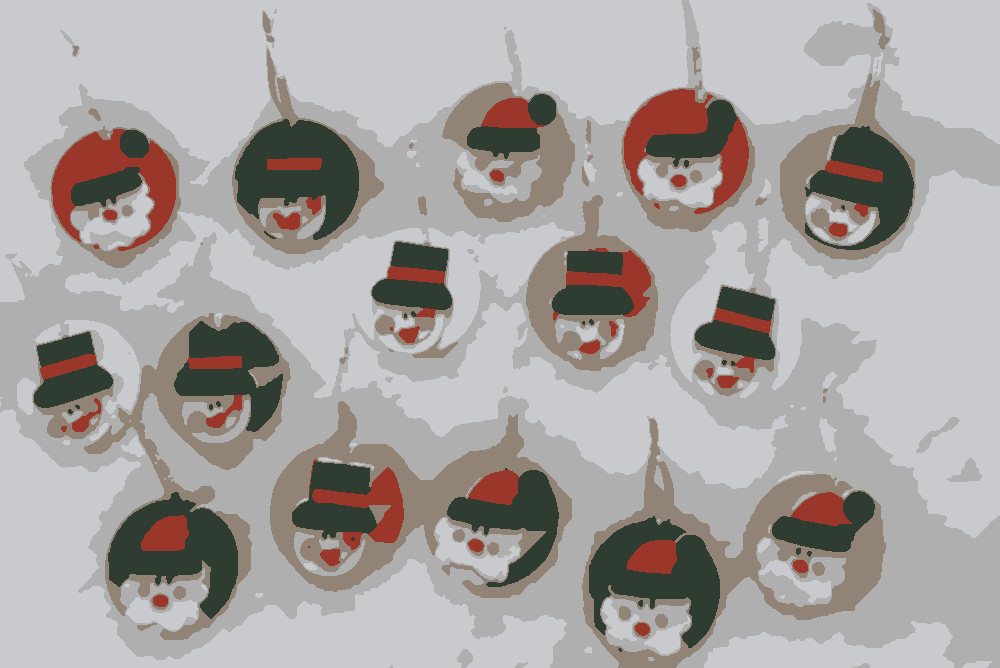
\includegraphics[width=6cm]{./imgkmeanscluster05-01.png}\\
\end{figure}
\end{center}
\begin{center}
\begin{figure}[H]
\centering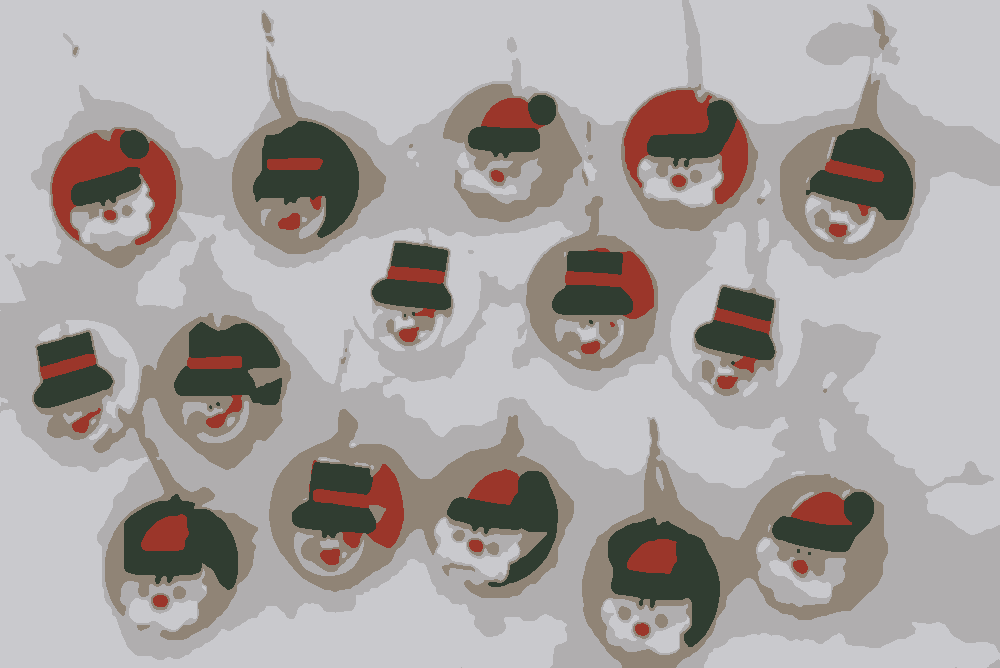
\includegraphics[width=6cm]{./imgkmeanscluster05-02.png}
\centering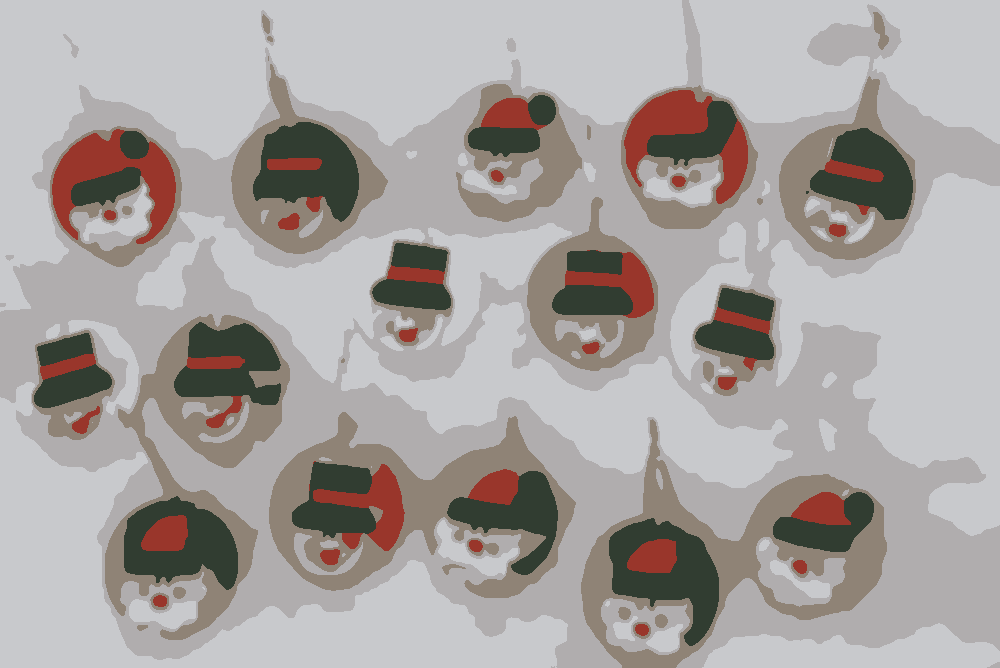
\includegraphics[width=6cm]{./imgkmeanscluster05-03.png}\\
\end{figure}
\end{center}
\begin{center}
\begin{figure}[H]
\centering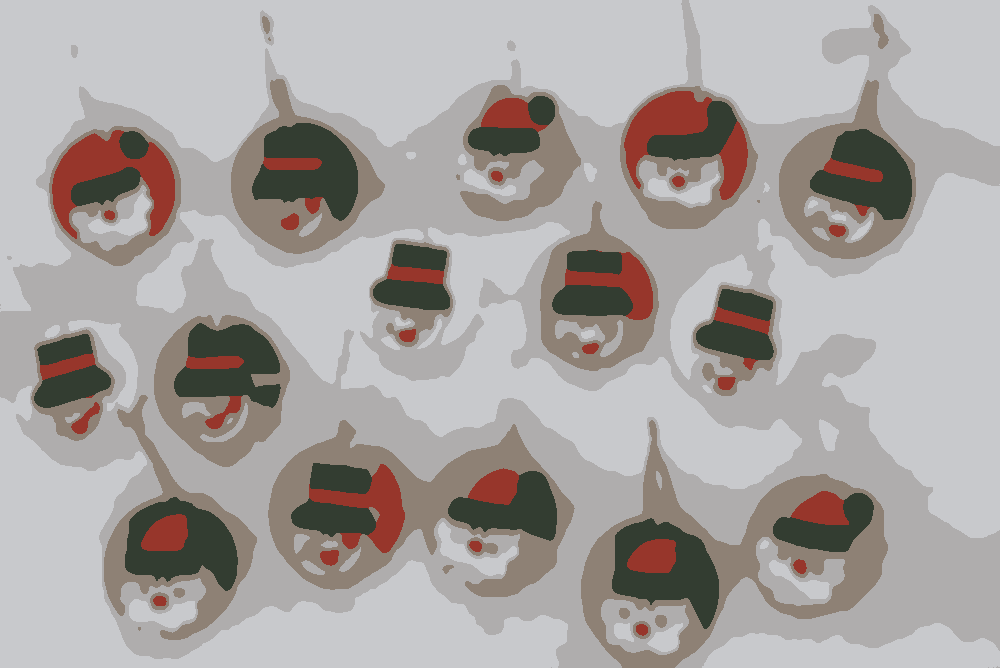
\includegraphics[width=6cm]{./imgkmeanscluster05-04.png}
\centering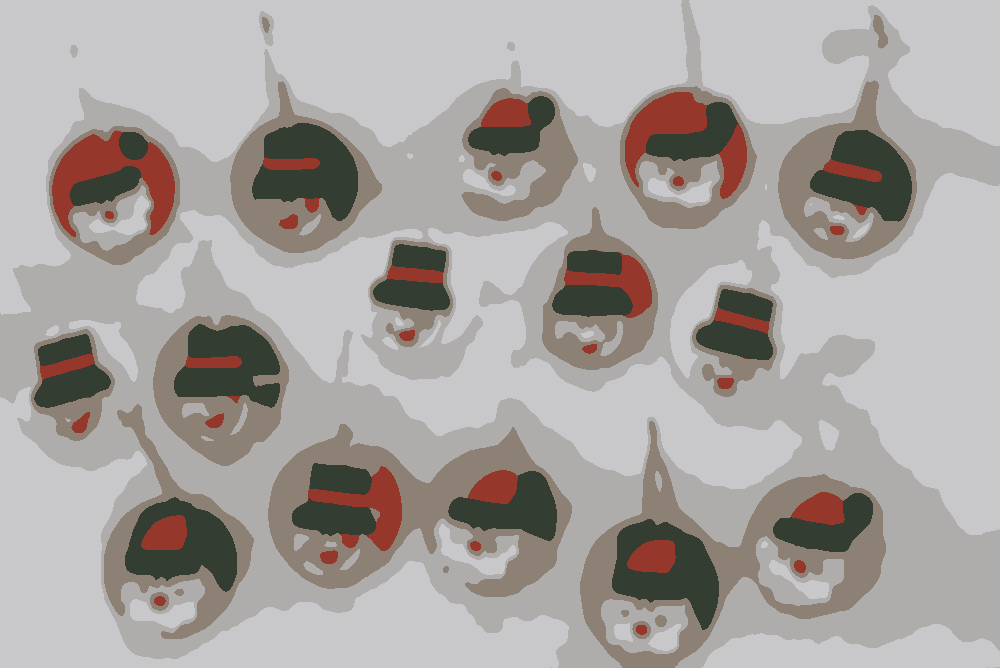
\includegraphics[width=6cm]{./imgkmeanscluster05-05.png}\\
\end{figure}
\end{center}
K=6:\\
\begin{center}
\begin{figure}[H]
\centering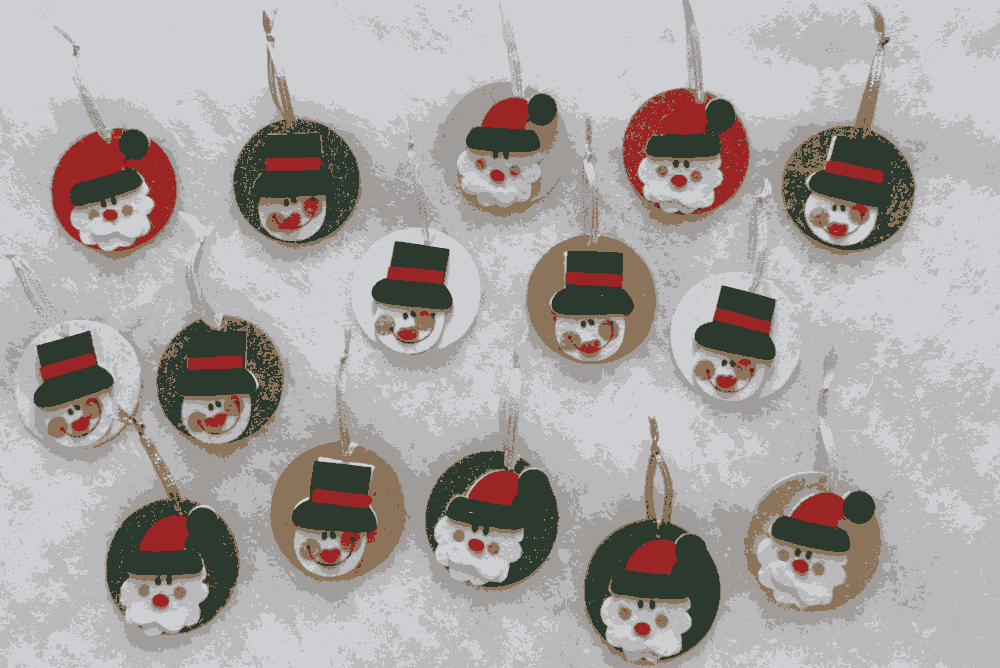
\includegraphics[width=6cm]{./imgkmeanscluster06-00.png}
\centering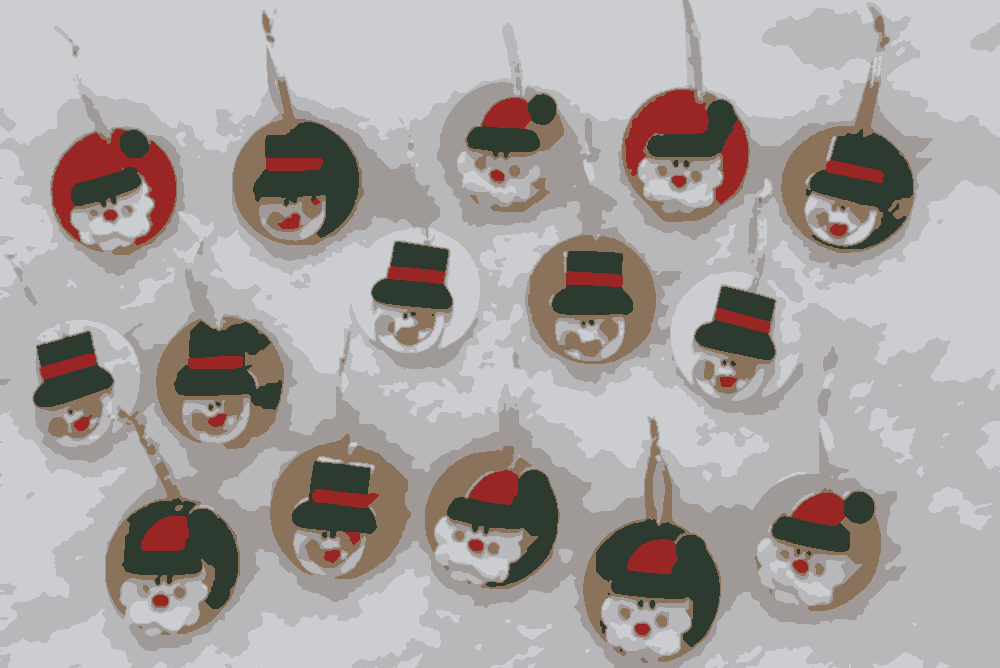
\includegraphics[width=6cm]{./imgkmeanscluster06-01.png}\\
\end{figure}
\end{center}
\begin{center}
\begin{figure}[H]
\centering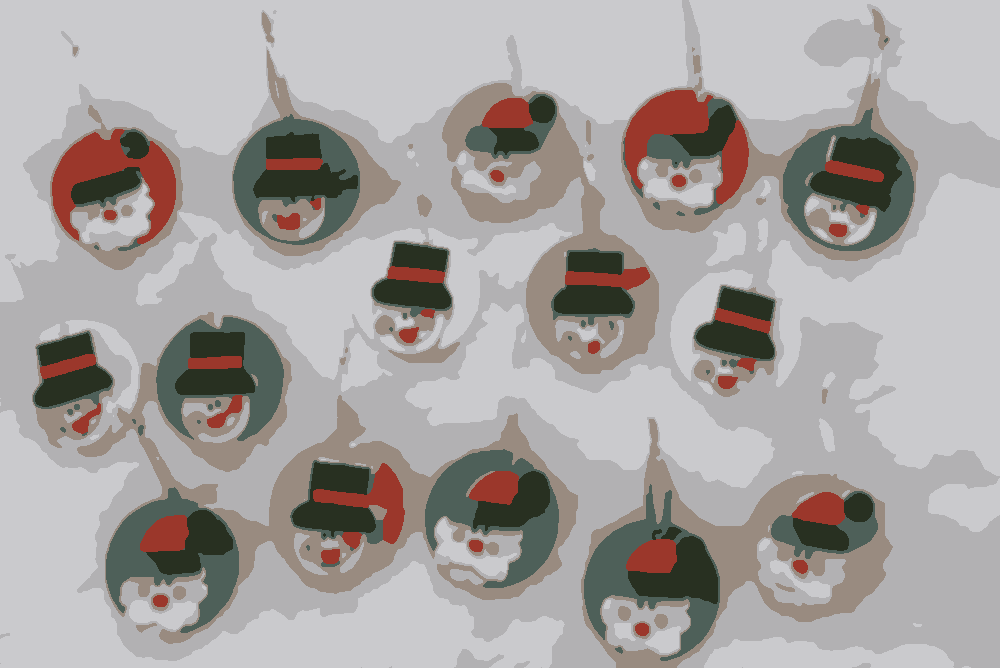
\includegraphics[width=6cm]{./imgkmeanscluster06-02.png}
\centering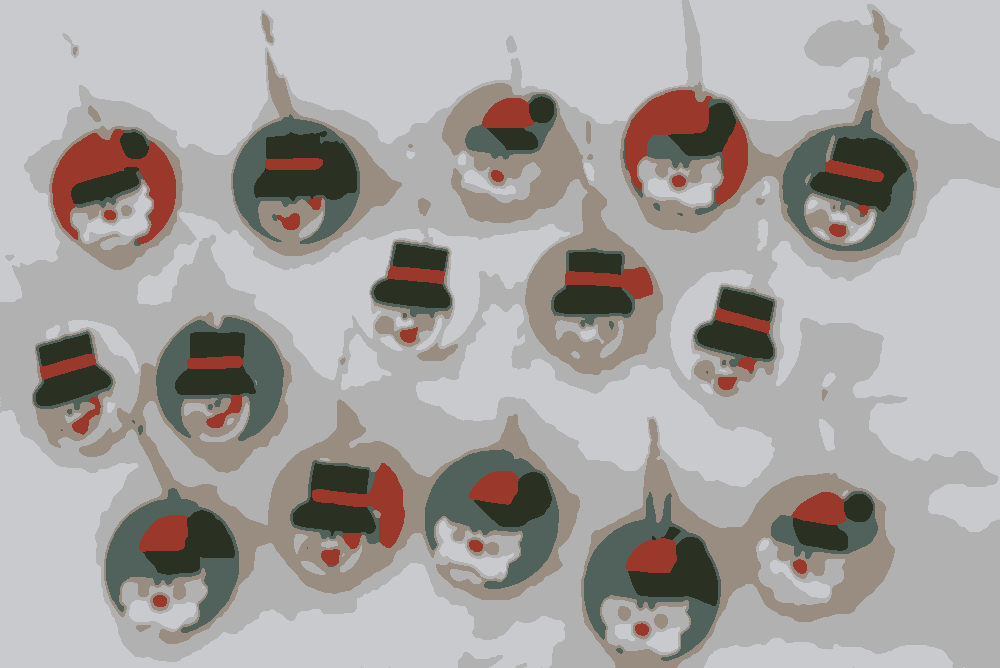
\includegraphics[width=6cm]{./imgkmeanscluster06-03.png}\\
\end{figure}
\end{center}
\begin{center}
\begin{figure}[H]
\centering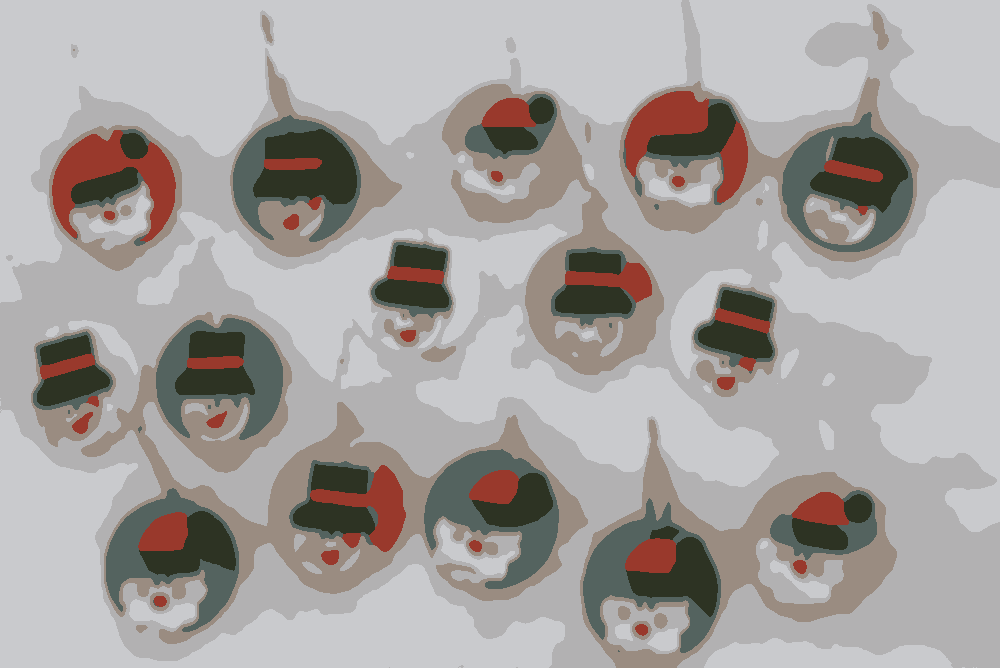
\includegraphics[width=6cm]{./imgkmeanscluster06-04.png}
\centering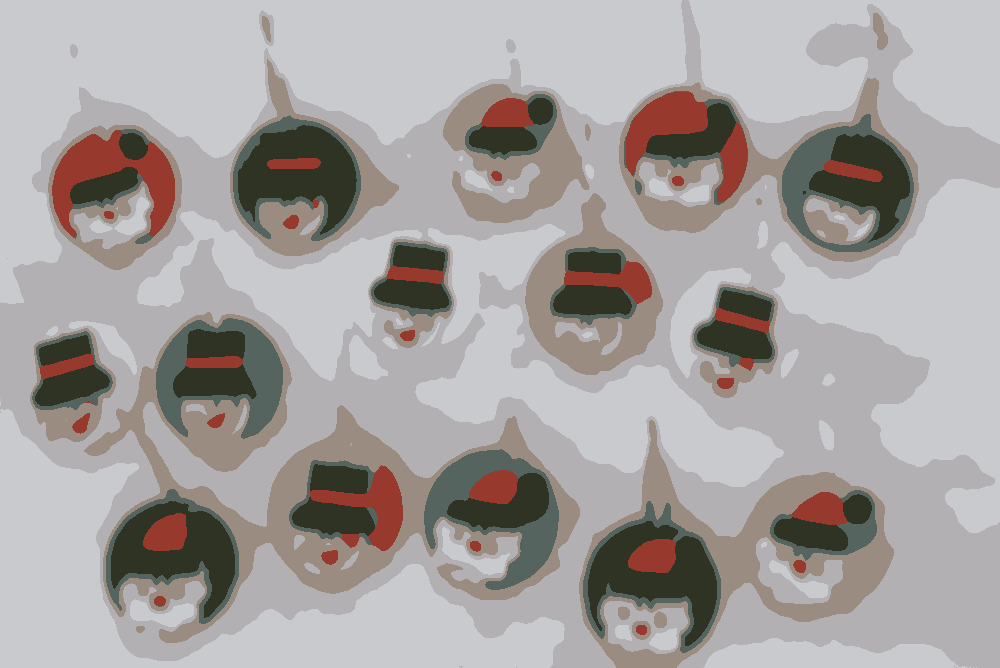
\includegraphics[width=6cm]{./imgkmeanscluster06-05.png}\\
\end{figure}
\end{center}

